\documentclass[12pt,border=0pt]{standalone}

\usepackage[utf8]{inputenc} 
\usepackage{amssymb,amsmath}
\usepackage{tikz}

\usepackage{nicefrac}


\thispagestyle{empty}

\begin{document}

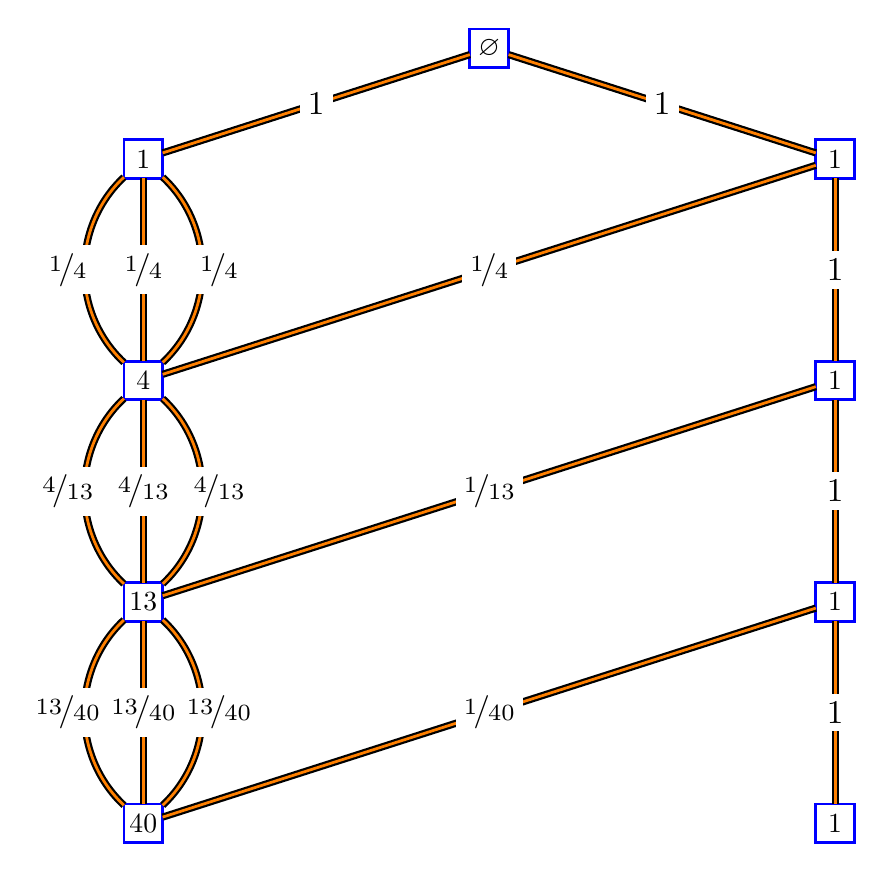
\begin{tikzpicture}[x=10pt,y=8pt]
  \centering
  \tikzset{VertexStyle/.style = {
    shape         = rectangle,
    draw          = blue, 
    fill          = white, 
  	line width    = 1pt, 
    text          = black,
    inner sep     = 1pt,
    outer sep     = 0pt,
    minimum size  = 14 pt,
    scale         = 1
    }
  }
  \tikzset{EdgeStyle/.style = {
    draw            = black, 
    thick,
    double          = orange,
    double distance = 1pt
    }
  }
  \tikzset{EdgeLabelStyle/.style = {
    %draw          = black,
    draw=white,
  	shape         = rectangle, % circle, 
  	line width    = 1pt, 
  	minimum size  = 1pt, 
    inner sep     = 2pt,
    outer sep     = 0pt,
    fill          = white, %yellow,
    text          = black,
    scale         = 1.2
    }
  }

	\node[VertexStyle](A1) at (25, 40) {$\varnothing$};
	\node[VertexStyle](B1) at (12.5, 35) {$1$};
	\node[VertexStyle](B2) at (37.5, 35) {$1$};
	\node[VertexStyle](C1) at (12.5, 25) {$4$};
	\node[VertexStyle](C2) at (37.5, 25) {$1$};
	\node[VertexStyle](D1) at (12.5, 15) {$13$};
	\node[VertexStyle](D2) at (37.5, 15) {$1$};
	\node[VertexStyle](E1) at (12.5, 5) {$40$};
	\node[VertexStyle](E2) at (37.5, 5) {$1$};
	\draw[EdgeStyle](A1) to node[EdgeLabelStyle]{$1$} (B1);
	\draw[EdgeStyle](A1) to node[EdgeLabelStyle]{$1$} (B2);
	\draw[EdgeStyle, bend left=-47](B1) to node[EdgeLabelStyle, xshift=-5]{$\nicefrac{1}{4}$} (C1); %label={below:#1}
	\draw[EdgeStyle, bend left=0](B1) to node[EdgeLabelStyle]{$\nicefrac{1}{4}$} (C1);
	\draw[EdgeStyle, bend left=47](B1) to node[EdgeLabelStyle, xshift=5]{$\nicefrac{1}{4}$} (C1);
	\draw[EdgeStyle](B2) to node[EdgeLabelStyle]{$\nicefrac{1}{4}$} (C1);
	\draw[EdgeStyle](B2) to node[EdgeLabelStyle]{$1$} (C2);
	\draw[EdgeStyle, bend left=-47](C1) to node[EdgeLabelStyle, xshift=-5]{$\nicefrac{4}{13}$} (D1);
	\draw[EdgeStyle, bend left=0](C1) to node[EdgeLabelStyle]{$\nicefrac{4}{13}$} (D1);
	\draw[EdgeStyle, bend left=47](C1) to node[EdgeLabelStyle, xshift=5]{$\nicefrac{4}{13}$} (D1);
	\draw[EdgeStyle](C2) to node[EdgeLabelStyle]{$\nicefrac{1}{13}$} (D1);
	\draw[EdgeStyle](C2) to node[EdgeLabelStyle]{$1$} (D2);
	\draw[EdgeStyle, bend left=-47](D1) to node[EdgeLabelStyle, xshift=-5]{$\nicefrac{13}{40}$} (E1);
	\draw[EdgeStyle, bend left=0](D1) to node[EdgeLabelStyle]{$\nicefrac{13}{40}$} (E1);
	\draw[EdgeStyle, bend left=47](D1) to node[EdgeLabelStyle, xshift=5]{$\nicefrac{13}{40}$} (E1);
	\draw[EdgeStyle](D2) to node[EdgeLabelStyle]{$\nicefrac{1}{40}$} (E1);
	\draw[EdgeStyle](D2) to node[EdgeLabelStyle]{$1$} (E2);

  \end{tikzpicture}

\end{document}
